\documentclass[letterpaper,10pt]{article}

\usepackage{titling}
\usepackage{listings}
\usepackage{url}
\usepackage{setspace}
\usepackage{subfig}
\usepackage{sectsty}
\usepackage{pdfpages}
\usepackage{colortbl}
\usepackage{multirow}
\usepackage{multicol}
\usepackage{relsize}
\usepackage{amsmath}
\usepackage{wasysym}
\usepackage{fancyvrb}
\usepackage{amssymb}
\usepackage{ifsym}
\usepackage{amsmath,amssymb,amsthm,graphicx,xspace}
\usepackage[titlenotnumbered,noend,noline]{algorithm2e}
\usepackage[compact]{titlesec}
\usepackage{XCharter}
\usepackage[T1]{fontenc}
\usepackage{tikz}
\usetikzlibrary{arrows,automata,shapes,trees,matrix,chains,scopes,positioning,calc}
\tikzstyle{block} = [rectangle, draw, fill=blue!20, 
    text width=2.5em, text centered, rounded corners, minimum height=2em]
\tikzstyle{bw} = [rectangle, draw, fill=blue!20, 
    text width=4em, text centered, rounded corners, minimum height=2em]

\definecolor{namerow}{cmyk}{.40,.40,.40,.40}
\definecolor{namecol}{cmyk}{.40,.40,.40,.40}

\let\LaTeXtitle\title
\renewcommand{\title}[1]{\LaTeXtitle{\textsf{#1}}}


\newcommand{\handout}[5]{
  \noindent
  \begin{center}
  \framebox{
    \vbox{
      \hbox to 5.78in { {\bf ECE356: Database Systems } \hfill #2 }
      \vspace{4mm}
      \hbox to 5.78in { {\Large \hfill #4  \hfill} }
      \vspace{2mm}
      \hbox to 5.78in { {\em #3 \hfill} }
    }
  }
  \end{center}
  \vspace*{4mm}
}

\newcommand{\lecture}[3]{\handout{#1}{#2}{#3}{Lecture #1}}
\newcommand{\tuple}[1]{\ensuremath{\left\langle #1 \right\rangle}\xspace}

\addtolength{\oddsidemargin}{-1.000in}
\addtolength{\evensidemargin}{-0.500in}
\addtolength{\textwidth}{2.0in}
\addtolength{\topmargin}{-1.000in}
\addtolength{\textheight}{1.75in}
\addtolength{\parskip}{\baselineskip}
\setlength{\parindent}{0in}
\renewcommand{\baselinestretch}{1.5}
\newcommand{\term}{Winter 2018}

\singlespace


\begin{document}

\lecture{ 23 --- Deadlock, Lock Granularity }{\term}{Jeff Zarnett}

\section*{Deadlock}

You should recall from learning about concurrency what deadlock is about, and therefore a brief review only is in order. Those in need of a refresher are advised to take a look through previous courses' material to get caught up. Others may find this to be review material, but it does deviate in some significant ways from the discussion of deadlocked processes.

We have already introduced the subject of deadlock and gave an informal definition as all transactions being ``stuck'' (unable to proceed). A more formal definition is given in~\cite{osi} (but modified for a database): ``the \textit{permanent} blocking of a set of transactions that either compete for system resources or communicate with each other''. There is emphasis on permanent. It may be possible for all transactions to be stuck temporarily, because one is waiting for some event (e.g., a read from disk), but this situation will resolve itself and is not deadlock. A set of transactions is truly deadlocked when each transaction in the set is blocked on some event that can only be triggered by another blocked transaction in the set. In this case it is permanent, because none of the events can take place.

Remember, there are four conditions necessary for a deadlock to take place:

\begin{enumerate}
	\item \textbf{Mutual Exclusion}: A resource belongs to, at most, one transaction at a time.
	\item \textbf{Hold-and-Wait}: A transaction that is currently holding some resources may request additional resources and may be forced to wait for them.
	\item \textbf{No Preemption}: A resource cannot be ``taken'' from the transaction that holds it; only the transaction currently holding that resource may release it.
	\item \textbf{Circular-Wait}: A cycle in the resource allocation graph.
\end{enumerate}

We could choose not to handle deadlock. This option is certainly convenient for database system designers: we simply pretend that deadlock can never happen, or if it does happen, it is the application developers' fault. While it is tempting and easy to just define a problem as being nothing we need to deal with, that's unrealistic in reality. If two transactions get deadlocked, the user may simply see no progress and just feel bad about it. But sad users are not a good thing, now, are they?

Although in theory it would be nice to prevent deadlock from ever occurring, in practice it is probably more likely that we will simply try to detect it and deal with it if it occurs. But prevention is worth looking at.

\subsection*{Deadlock Prevention}

 The first three conditions for deadlock (mutual exclusion, hold and wait, and no preemption) are all necessary for deadlock to be possible. If we eliminate one of these three pillars, deadlock is not possible and it is prevented from happening. If we prevent the circular wait from occurring, we are still in a world where deadlock can occur but we cleverly avoid it taking place based on how we allow locks to occur.

\paragraph{Mutual Exclusion.} This pillar cannot, generally speaking, be disallowed. The purpose of  mutual exclusion is to prevent errors like inconsistent state or crashes. Getting rid of mutual exclusion to rule out the possibility of deadlock is a cure that is worse than the disease. It is therefore not acceptable as a solution.

\paragraph{Hold and Wait.} To prevent the hold-and-wait condition, we must guarantee that when a transaction requests a resource, it does not have any other resource. One plausible solution is that the transaction must request all resources at the beginning of the program. So if the program is going to need resources $R_{1}$, $R_{2}$, and $R_{3}$ at some point in the program, all three must be requested right at the beginning and held throughout the transaction. No further resources may be requested at any time during execution~\cite{osc}.

When talking about processes, actually we said this requires some amount of clairvoyance: a process has to know in advance all of the resources that it will need. Remember that a file is a resource, and even a simple program like a text editor can be used by the user to open an arbitrary file; how do we know in advance which will be requested? But with database transactions, actually, we can actually evaluate what data items are needed. That might not be trivial, but at least for databases it is possible.

This also has performance implications: a transaction cannot start until it has all the resources it will ever need, even if it will not need them until much later. Thus, transactions might spend a lot of time waiting before starting; something that users may not tolerate. In theory, a transaction might never start if one or more of the resources it needs is always in use (so this is vulnerable to starvation).
 


\paragraph{No Preemption.} If we violate this condition, it means that we do have preemption: forcible removal of resources from a transaction. In the database context, if we have to preempt a transaction, it means the transaction in question is rolled back and then restarted. To work out an ordering, transactions are assigned a timestamp. If a transaction is rolled back, its timestamp remains the same~\cite{dsc}. There are two approaches for what happens if we need to do pre-emption:

The first is called \textit{wait-die}: if a transaction $T_{i}$ requests an item held by $T_{j}$, then the timestamps of these two transactions are compared. $T_{i}$ will be allowed to wait if it is older (i.e. its timestamp is a smaller number) than $T_{j}$, otherwise it ``dies'' (is rolled back). 

The second is \textit{wound-wait}: if a transaction $T_{i}$ requests an item held by $T_{j}$, then the timestamps of these two transactions are compared. If $T_{i}$ is the younger transaction (its timestamp is larger), then $T_{i}$ can wait. Otherwise, $T_{j}$ is ``wounded'' by $T_{i}$ and $T_{j}$ is rolled back.

So, in case of a conflict, one of the two transactions is going to be rolled back. And it is always the younger one. This is not because older transactions vote in higher numbers, but because it tends to be more expensive to restart an older transaction. A transaction that has been running for a long time, if it is restarted, has to do a lot more work to get to the point where it was terminated than a younger transaction. Another reason: if the oldest transaction were constantly the one selected, that transaction itself might never get to run to completion (starvation) because it is constantly killed before it finishes. A third reason is somewhat more subtle: if the killing transaction is very aggressive then perhaps no tasks run to completion because each transaction, shortly after becoming the oldest, is claimed by the deadlock recovery transaction. Therefore, young transactions tend to be the ones selected.

In either approach there may be unnecessary rollbacks~\cite{dsc}.

Instead we could also have locks that have timeouts: when a lock is requested there is a defined maximum time the transaction is willing to wait. If that time limit is reached, the transaction rolls back automatically and begins again. The obvious difficulty lies in choosing the length of time that the transactions will wait: too long and a deadlock persists for a lengthy period of time; too short and transactions do not complete because they are rolled back repeatedly. And that is generally unfortunate. This sort of approach is not especially recommended. 

\paragraph{Circular Wait.}
We have already discussed the idea of using two phase locking to put an ordering on the locks and we need not repeat that yet again. 

\subsection*{Deadlock Detection}

In previous courses you may have covered algorithms like the banker's algorithm and the graph algorithm for detecting deadlock. It is the second one that is interesting in the database.

A quick review of the graph algorithm follows, then. If resources have only a single instance, we may reduce the graph to a simplified version called the \textit{wait-for} graph. This removes the resource boxes from the diagram and indicates that a process $P_{i}$ is waiting for process $P_{j}$ rather than for a resource $R_{k}$ that happens to be held by $P_{j}$. An edge $P_{i} \rightarrow P_{j}$ exists in the wait-for graph if and only if the resource allocation graph has a request $P_{i} \rightarrow R_{k}$ and an assignment edge $R_{k} \rightarrow P_{j}$~\cite{osc}. Consider the example below:

\begin{center}
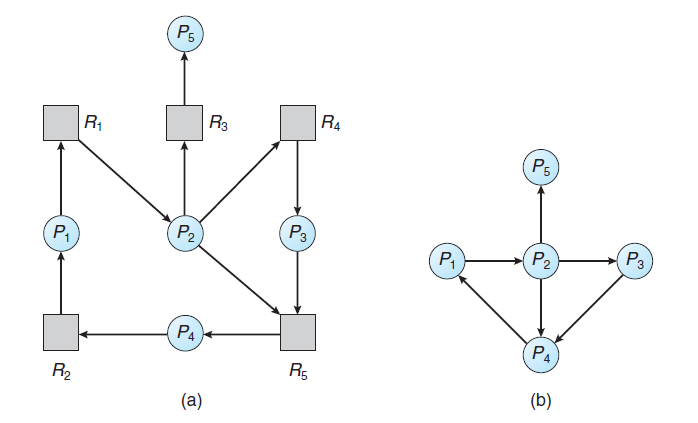
\includegraphics[width=0.5\textwidth]{images/rag-waitfor.png}\\
(a) A resource allocation graph and (b) its corresponding wait-for graph~\cite{osc}.
\end{center}

Because locks are unique (there is always only one instance) then there is no need to use the resource allocation graph and we can always use the simplified wait-for graph for transactions as below:

\begin{center}
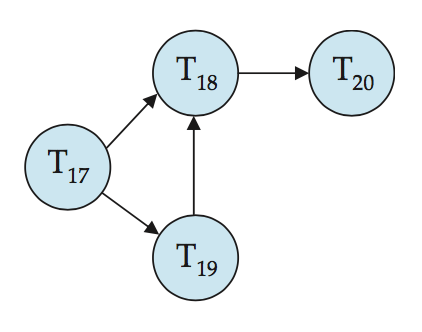
\includegraphics[width=0.25\textwidth]{images/transaction-waitfor.png}\\
Transaction wait-for graph~\cite{dsc}.
\end{center}


Given the wait-for graph, it is trivial for humans to look at this and determine if there is a cycle, but for the computer it takes slightly more work. We must execute an algorithm to determine if there is a cycle. A cycle exists in the wait for graph if and only if a deadlock exists in the system. Such cycle detection algorithms tend to have runtime characteristics of $\Theta(n^{2})$ where $n$ is the number of nodes in the graph. Though not a formal proof and probably not acceptable to write on a data structures and algorithms examination, the premise of the algorithm is: for each node $n$ in the graph, examine each possible path from that node. If a node is reached from which no further path is available, examine the next path. If node $n$ is reached on the current path, a cycle is detected and the algorithm terminates. 

The runtime characteristic of the simple deadlock detection algorithm was identified as $\Theta(n^{2})$. This means that the deadlock detection routine is expensive to execute.

This prompts a question: how often should the deadlock detection algorithm be run? One strategy is to run it every time a resource is requested. Running the algorithm might be rather expensive, so perhaps this is too often. An obvious optimization: it should only run every time a resource request cannot be granted (that is, a transaction is waiting). Another idea: run it periodically instead.

When to run the deadlock detection algorithm depends on how often we expect deadlock to occur, and how severe a problem it is when deadlock occurs. If deadlock happens a lot, checking for deadlock often will make sense. If the consequences of a deadlock are severe, it makes sense to check frequently to identify the problem as soon as possible.

\subsection*{Deadlock Recovery}

It is clear that our recovery strategy in the database context is rollback. But rather than just simply rolling transactions back and restarting them. 

On the subject of what transaction to select as a victim we already identified the timestamp as one possible way to decide, but there exist a number of other possible criteria~\cite{dsc}:

\begin{enumerate}
\item How long the process has been executing.
	\item How long is remaining in execution (see the estimates from the execution plan).
	\item What resources the process has used.
	\item Future resource requests, if known.
	\item How many times, if any, the process has been selected as a victim (to prevent starvation).
\end{enumerate}

After a victim has been selected, we might reason, it's pretty easy from here: simple roll that transaction back. That would be a total rollback: undo all the steps of the transaction and start from the beginning once again. There exists, however, the ability to do a \textit{partial rollback}. 

The goal of the partial rollback is to rollback the transaction back only as much as is necessary to break the deadlock;  this is accomplished by maintaining the sequence of lock requests and grants. By finding the lock(s) that are implicated in the deadlock, we can roll back a transaction to where it obtained the first of such locks~\cite{dsc}. This can be beneficial if the amount of work saved is large enough to outweigh the effort required to determine where the lock conflict occurs. For small transactions, a full restart is probably sensible; for longer ones it might be worth it to try to do a partial rollback instead.

\section*{Lock Granularity}

\bibliographystyle{alphaurl}
\bibliography{356}


\end{document}
